\chapter{Orbifolds}

\scribe{Roger Ten}

\section{Defining an orbifold}

In this section $X$ denotes a topological space and $G$ denotes a topological group. So must begin by defining what is a topological group.

\begin{defn}
\begin{enumerate}
\item A \emph{topological group} is a topological space that is simultaneously a group such that, the group operations are continuous.
\item A topological space $X$ is called \emph{$G$-space} if a topological group $G$ acts on $X$ via a continuous map
 $G\times X \longrightarrow X$, $(g,x)\longmapsto gx$ such that
  $g(hx)=(gh)x$ and $1_Gx=x$.
\end{enumerate}
\end{defn}

\begin{example}
\begin{itemize}
  \item Lie groups: $O(n), SO(n)$
  \item $S^1$ is a topological space and it is also a group via:
  $$\begin{array}[c]{cccc}
 +: &S^1\times S^1&{\rightarrow}&S^1\\
&(\varphi,\psi)&{\rightarrow}& \varphi +\psi
\end{array}$$
\begin{center}
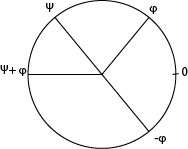
\includegraphics[width=0.5\textwidth]{./suma}
\end{center}
\end{itemize}

\end{example}

Now is coming a list of definitions
\begin{defn}
Let  $x\in X$ be a point.
\begin{enumerate}
\item $G_x=\{g\in G : gx=x\}=Stab_G(x)$ is called the \emph{stabilizer of $x$} or the isotropy subgroup of $x$. $G_x$ is a subgroup of $G$ $(G_x\leqslant G).$
\item $G(x)=\{gx : g\in G\}\subset X$ is the \emph{orbit of $x$}.
\item The action of $G$ on $X$ is \emph{free} if $G_x=\{ 1\} \forall x\in X.$
\item The action of $G$ on $X$ is \emph{transitive} if $G(x)=X \forall x\in X$, i.e., there exist only one orbit.
\item The map $G/G_x\rightarrow G(x)$ is a continuous bijection
\item The orbit space $X/G$ is the set of all orbits in $X$. (It is a topological space with quocient topology).
\item A map $f:X\rightarrow Y$ of $G$-spaces is \emph{$G$-equivariant} (or $G$-map) if $f(gx)=g(f(x)); g\in G$. so the following diagram commutes:
 $$\begin{array}[c]{ccc}
X&\stackrel{f}{\rightarrow}&Y\\
\downarrow\scriptstyle{g}&\circlearrowright&\downarrow\scriptstyle{g}\\
X&\stackrel{f}{\rightarrow}&Y
\end{array}$$
\end{enumerate}
\end{defn}

%---------------------------------------------------- Orbifold Chart

\begin{defn}
An \emph{orbifold chart} on a topological space $X$ is tuple $(\tU,G,\cU, \pi)$, such that:
\begin{itemize}
  \item $\cU\subset X$ is an open subset (neighborhood).
  \item $\tU\subset \RR^n$ is an open subset.
  \item $G$ is a finite group of homomorphisms of  $\tU$.
  \item $\pi:\tU\rightarrow \cU$ can be factorized as $\pi=\tilde{\pi}\circ p$, where 
  $p:\tU\rightarrow \tU/G$ is the orbit map and $\tilde{\pi}:\tU/G\rightarrow \tU$ is an homomorphism.
\end{itemize}
\end{defn}





\begin{tikzpicture}[>=angle 90]
\matrix[matrix of math nodes,row sep=3em, column sep=0.25em,
text height=1.5ex, text depth=0.25ex]
{G&\underset{act\ on}{\circlearrowleft} &|[name=tU]| \tU &\subset &\RR^n \\
     &    &           & &|[name=tUG]| \tU/G \\
& & |[name=U]| \cU & \subset &X \\};
\draw [->,font=\scriptsize]
(tU) edge node[auto] {$p$} (tUG)
(tU) edge node[auto] {$\pi$} (U)
(tUG) edge node[auto] {$\tilde{\pi}$} (U);
\end{tikzpicture}

 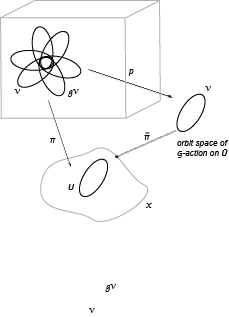
\includegraphics[width=0.5\textwidth]{orbitchart}



 \begin{defn} Two orbifold charts are \emph{compatible} if for all $\tilde{u_i}\in \tU_i,
   i=1,2$ such that $\pi_1(\tilde{u_1})=\pi_2(\tilde{u_2})$ there exists a homomorphism
   $h:\tV_1\rightarrow\tV_2$, where $\tV_i$ is a neighborhood of $\tilde{u_i}$ in $\tU_i$,
   such that $\pi_1=\pi_2\circ h$ on $\tV_1$

\begin{center}
\begin{tikzpicture}[>=angle 90]
\matrix[matrix of math nodes,row sep=1em, column sep=0.5em,
text height=1.5ex, text depth=0.25ex]
{|[name=U2]|\tU_2&\supset &|[name=V2]| \tV_2 & &|[name=V1]|\tV_1&\subset &|[name=U1]| \tU_1 \\
&&&\circlearrowright &&&\\
|[name=U2G]|\tU_2/G& & &|[name=U1U2]| \tU_1\cap\tU_2 & & &|[name=U1G]| \tU_1/G0\\};
\draw [->,font=\scriptsize]
(V1) edge node[auto] {$h$} (V2)
(V1) edge node[auto] {$\pi_1$} (U1U2)
(V2) edge node[auto] {$\pi_2$} (U1U2)
(U1G) edge node[auto] {$\tilde{\pi}_1$} (U1U2)
(U2G) edge node[auto] {$\tilde{\pi}_2$} (U1U2)
(U1) edge node[auto] {$p_1$} (U1G)
(U2) edge node[auto] {$p_2$} (U2G);
\end{tikzpicture}
\end{center}
\end{defn}

\begin{remark}
$G_i=\{1\}$ yields manifolds.
\end{remark}

\begin{defn}
An \emph{orbifold atlas} is a collection of compatible orbifold charts that cover $X$.\\
An \emph{orbifold $Q$} is an underlying Hausdorff topological space $|Q|$ with an orbifold atlas.
\end{defn}

\section{Covering orbifolds}

A \emph{covering} of a topological space $X$ is a topological space $Y$, together with a
continuous surjective projection $\pi: Y\rightarrow X$ such that for every $x\in X$ exist
$\cU_x$ open neighborhood of $x$ such that the pre-image $\pi^{-1}(\cU_x)$ is a disjoint
union of copies of $\cU_x$.


\begin{defn}
A \emph{covering orbifold} of an orbifold $Q$ is an orbifold $\tilde{Q}$ with a projection $\pi:|\tilde{Q}|\rightarrow|Q|$ between the underlying spaces with the following property:
\begin{quote}
  For any $x\in |Q|$ there exist a neighborhood $\cU\cong \tU/G$; $\cU\subset \RR^n$ such
  that each connected component $C$ of $\pi^{-1}(\cU)$ is homeomorphism to $\tU/\Gamma_i$
  for some subgroup $\Gamma_i\leqslant G$.
\end{quote}
\end{defn}
\begin{remark}
This homeomorphism $\varphi$ must respect both projections, namely $\pi$ and $p_i:\tU/G\rightarrow\tU/\Gamma_i$.

\vspace*{2cm}
\begin{tikzpicture}[>=angle 90]
\matrix[matrix of math nodes,row sep=1em, column sep=3em,
text height=1.5ex, text depth=0.25ex]
{&&&&\\
|[name=tQ]| |\tilde{Q}|&|[name=C]| 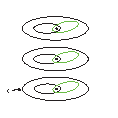
\includegraphics[width=0.15\textwidth]{./C} & &|[name=tU]|\tU &|[name=tUd]| 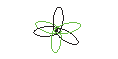
\includegraphics[width=0.15\textwidth]{./tU} \\
&&&&\\
 &&\circlearrowright & |[name=tUG]| \tU/G& |[name=tUGd]| \\
|[name=Q]| |Q|&|[name=U]|  \cU & & &
\includegraphics[width=0.15\textwidth]{./tUG} \\
&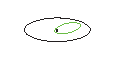
\includegraphics[width=0.15\textwidth]{./U}&&&\\};
\draw [->,font=\scriptsize]
(tQ) edge node[auto] {$\pi$} (Q)
(C) edge node[auto] {$\pi$} (U)
(tUG) edge node[auto] {$\tilde{\pi}$} (U)
(tU) edge node[auto] {$\varphi$} (C)
(tU) edge node[auto] {$p$} (tUG)
(tUd) edge node[auto] {$p$} (tUGd);
\end{tikzpicture}


\end{remark}

\begin{defn}
An orbifold is called \emph{good} or developable if there exists some manifold that covers it. Otherwise, it is \emph{bad} or not developable
\end{defn}



% Local Variables: 
% mode: latex
% TeX-master: "dag-upc"
% End: 
